% \documentclass[final]{article}
\documentclass{article}

\usepackage[final]{neurips_2025}

\usepackage{fontspec}
\setmainfont{Liberation Serif}
\setsansfont{Liberation Sans}
\usepackage{hyperref}
\usepackage{url}
\usepackage{booktabs}
\usepackage{amsfonts}
\usepackage{nicefrac}
\usepackage{microtype}
\usepackage{xcolor}
\usepackage{graphicx}
\usepackage{amsmath}
\usepackage{multirow}
\usepackage{caption}

\title{Data-Driven Sales Forecasting and Supply Chain Optimization for E-Commerce}

\author{%
  [K-ATM] \\
  % [Affiliation] \\
  \texttt{nhatminh010905@gmail.com} \\
}

\begin{document}

\maketitle

\begin{abstract}
Báo cáo phân tích hiệu quả kinh doanh của một công ty thương mại điện tử trong 10 năm (2012–2022), phát hiện mô hình "Vòng Xoáy Chết" do giảm giá quá mức gây xói mòn lợi nhuận, đồng thời đề xuất khung tối ưu hóa kép giúp giải phóng tới 180 triệu đồng vốn lưu động mỗi quý. Ngoài ra, nhóm xây dựng quy trình dự báo doanh thu và giá vốn hàng bán theo ngày bằng mô hình tổ hợp 12 thuật toán, đạt độ chính xác cao (R² > 0,99) và được kiểm chứng qua phân tích SHAP.
\end{abstract}

%==========================================================================
% PART 2: BUSINESS INSIGHTS
%==========================================================================

\setcounter{section}{2}
\setcounter{subsection}{0}

\section*{Phần 2: Business Insights}

\subsection{Descriptive Analytics: Bức tranh tổng quan về Lợi nhuận và Chi phí }

\begin{figure}[h]
  \centering
  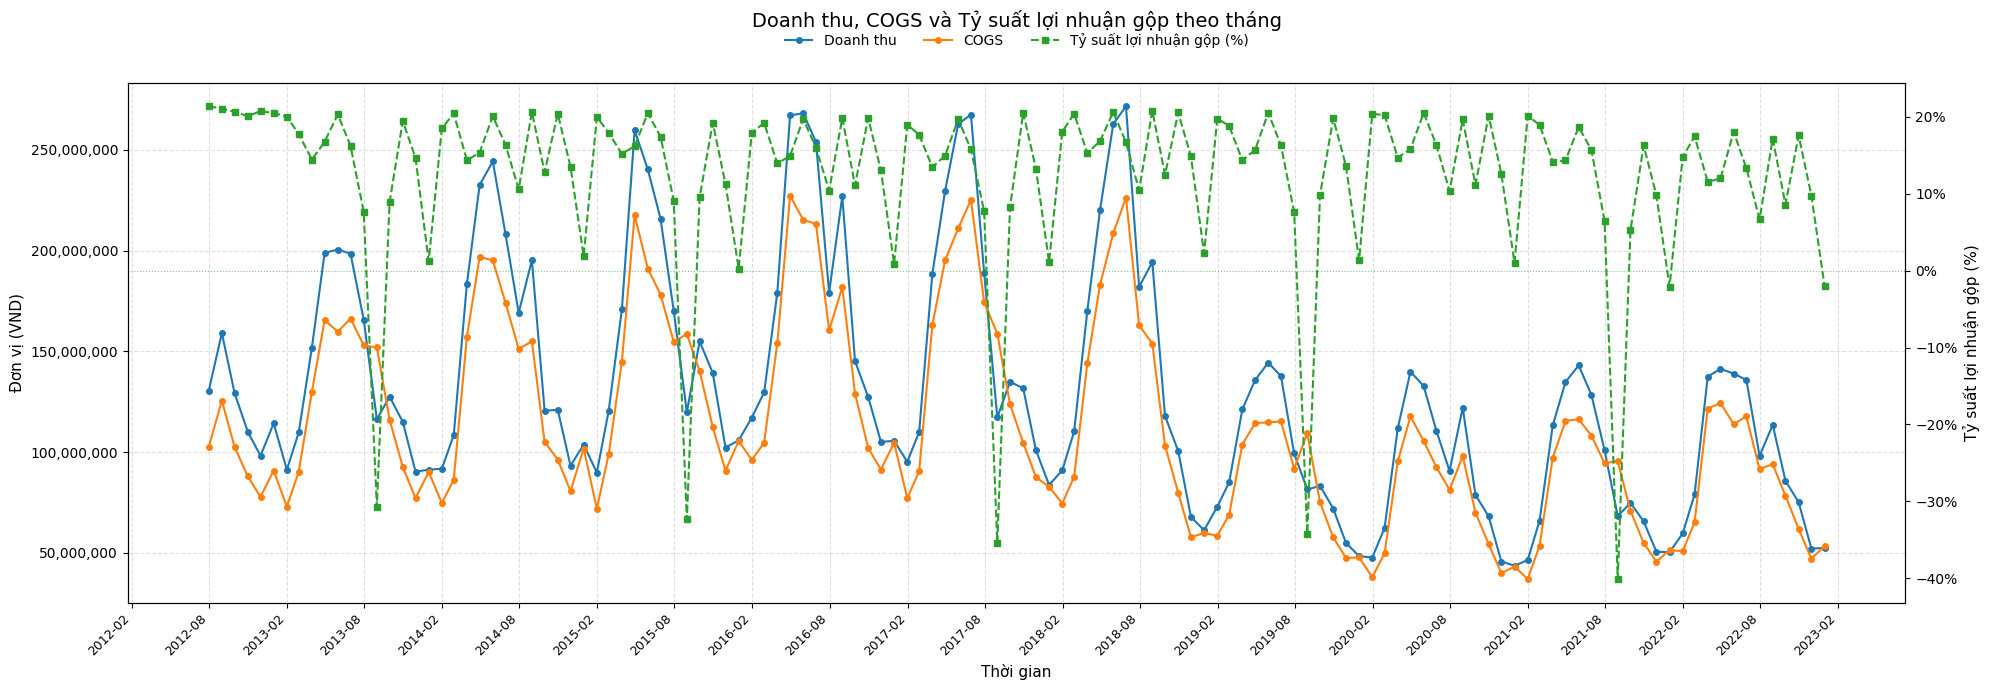
\includegraphics[width=0.85\linewidth]{part2.1.png}
  \caption{Biên lợi nhuận theo tháng (2012–2022)}
  \label{fig:margin}
\end{figure}

Phân tích các chỉ số tài chính cho thấy Gross Margin của doanh nghiệp đang bị kìm hãm ở mức tối đa 20\% và thường xuyên chạm đáy -40\% theo chu kỳ mùa vụ (tháng 10). Nguyên nhân cốt lõi đến từ việc COGS luôn duy trì tỷ trọng quá cao và doanh nghiệp liên tục lạm dụng các đợt chiết khấu sâu (đặc biệt vào tháng 8 và tháng 12 định kỳ mỗi 2 năm). Chính sách giảm giá này đẩy giá bán thực tế rớt mạnh, khiến biên lợi nhuận bốc hơi hoàn toàn về 0\% (vào tháng 12) và âm nặng từ -35\% đến -40\% (vào tháng 8). Việc một doanh nghiệp 10 năm tuổi vẫn phải chấp nhận hy sinh biên lợi nhuận để đổi lấy tăng trưởng doanh thu là tín hiệu báo động đỏ, đòi hỏi phải khẩn trương tối ưu lại cấu trúc SKU và chiến lược giá bán. 

\subsection{Diagnostic Analytics: Tỷ suất lợi nhuận gộp và lượng hàng tồn kho theo sản phẩm}

\begin{figure}[h]
  \centering
  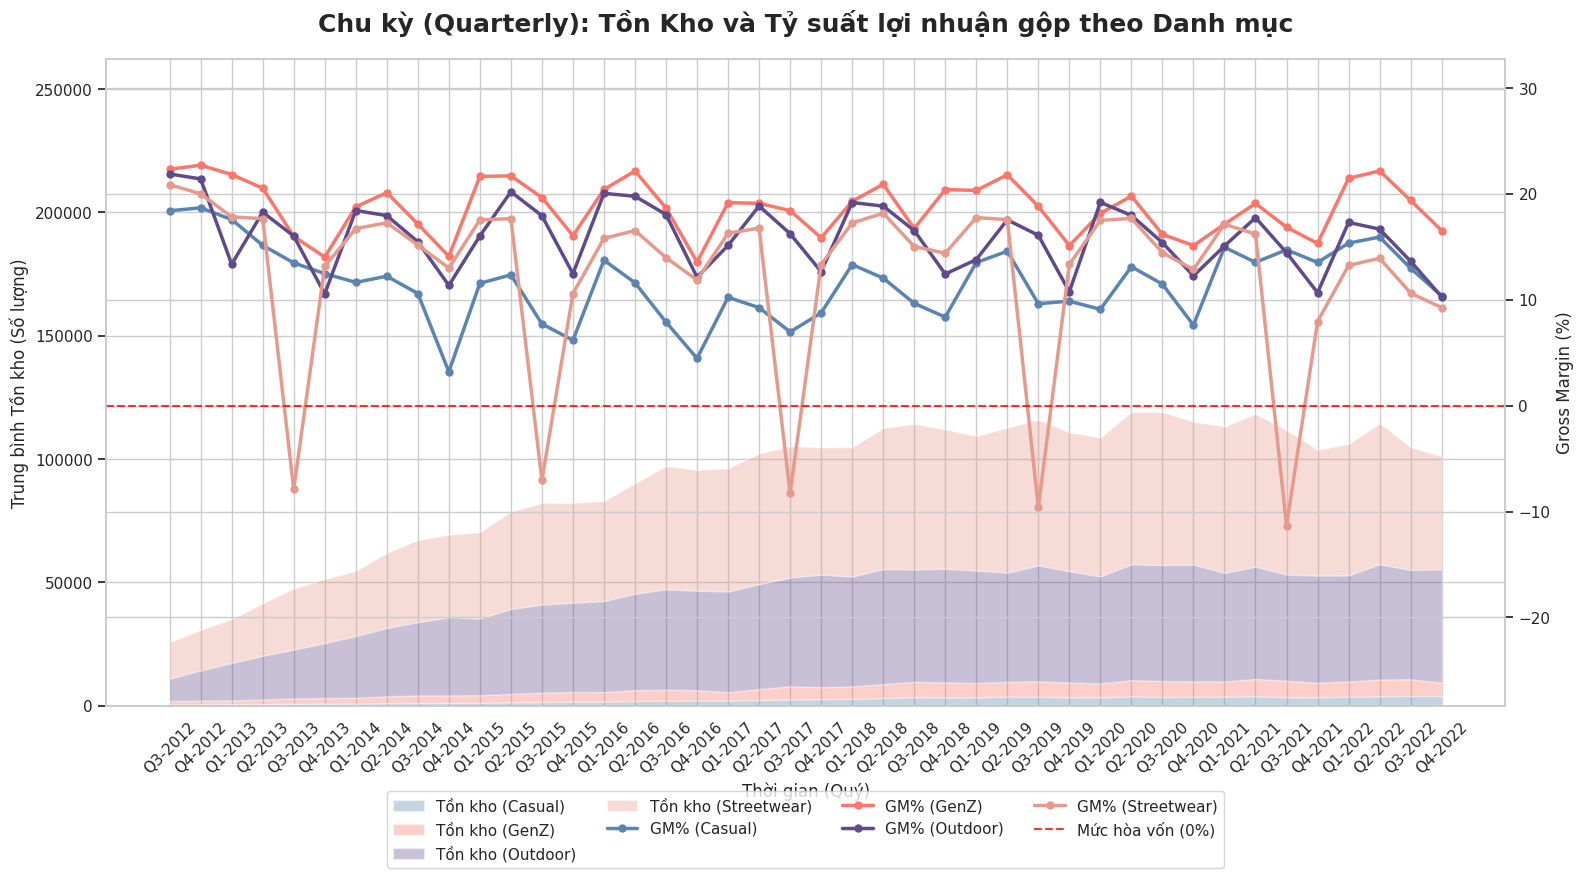
\includegraphics[width=0.85\linewidth]{part2.2.png}
  \caption{Tồn kho theo danh mục và biên lợi nhuận (2012–2022)}
  \label{fig:inventory}
\end{figure}

Để nhìn thấy rõ nét hơn tình hình kinh doanh của doanh nghiệp, nhóm đã đi sâu hơn vào các chu kỳ kinh doanh, hàng tồn theo các danh mục sản phẩm. Nhóm nhận thấy rằng điểm lớn nhất khiến cho biên lợi nhuận âm tháng 8 mỗi hai năm là từ chiến lược giảm giá quá mạnh, đặc biệt là những đợt khuyến mãi theo mùa, như tháng 8 và tháng 12. Điều này khiến cho chi phí vốn sản phẩm đã cao nay lại giảm thêm doanh thu, kéo theo biên lợi nhuận suy giảm xuống mức âm 10\% ở các quý II. 
Một điểm đặc biệt nữa là việc doanh nghiệp đang gặp vấn đề về việc tối ưu hàng tồn kho, việc danh mục Streetwear có lượng hàng tồn kho không những rất lớn (khoảng 100000 sản phẩm) mà còn khiến biên lợi nhuận thường âm mỗi tháng 8. Đây là một vấn đề rất nhức nhối cho doanh nghiệp, biên lợi nhuận đã âm, lượng tồn đã không được giải quyết hiệu quả.

\subsection{Diagnostic Analytics: Hiệu quả xả hàng tồn kho bằng chương trình khuyến mãi}

\begin{figure}[h]
  \centering
  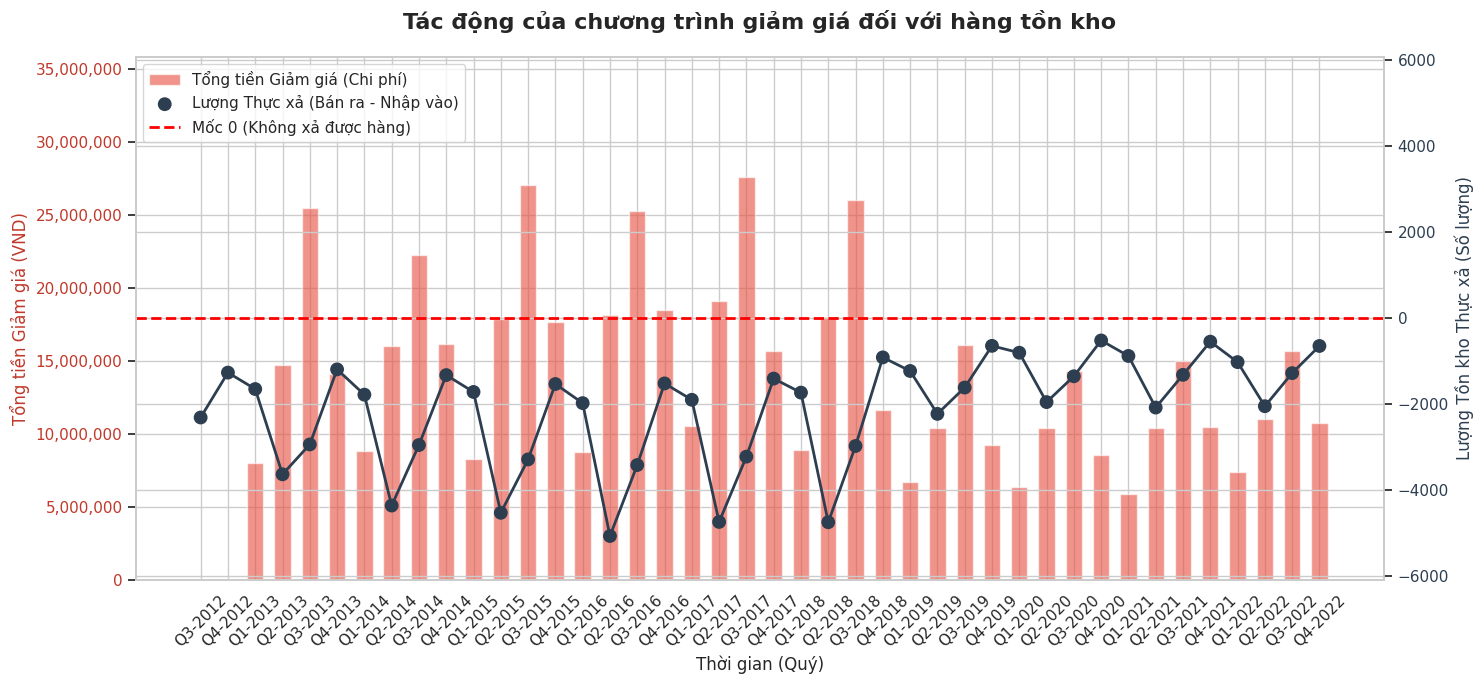
\includegraphics[width=0.85\linewidth]{part2.3.png}
  \caption{Nghịch lý doanh số và tồn kho (2012–2022)}
  \label{fig:paradox}
\end{figure}

Phân tích danh mục Streetwear bộc lộ một nghịch lý vận hành nghiêm trọng: suốt 10 năm, tồn kho thực xả luôn nằm dưới mốc 0 do khối lượng nhập mới liên tục vượt xa lượng bán ra. Bất chấp việc đầu tư ngân sách khổng lồ cho các đợt giảm giá sâu, đường tồn kho thực xả vẫn không được cải thiện và chưa từng một lần vượt lên mức dương. Sự đứt gãy giữa khâu Thu mua và Bán hàng đã vô hiệu hóa hoàn toàn chiến lược xả kho. Việc liên tục rơi vào tình trạng gánh lỗ kép – vừa bốc hơi biên lợi nhuận do chiết khấu, vừa kẹt cứng vốn lưu động – là minh chứng rõ nét cho một chuỗi cung ứng đang mất kiểm soát và thiếu bền vững. 

\subsection{Predictive Analytics: Dự báo vòng lặp tồn kho và khoản lỗ}

\begin{figure}[h]
  \centering
  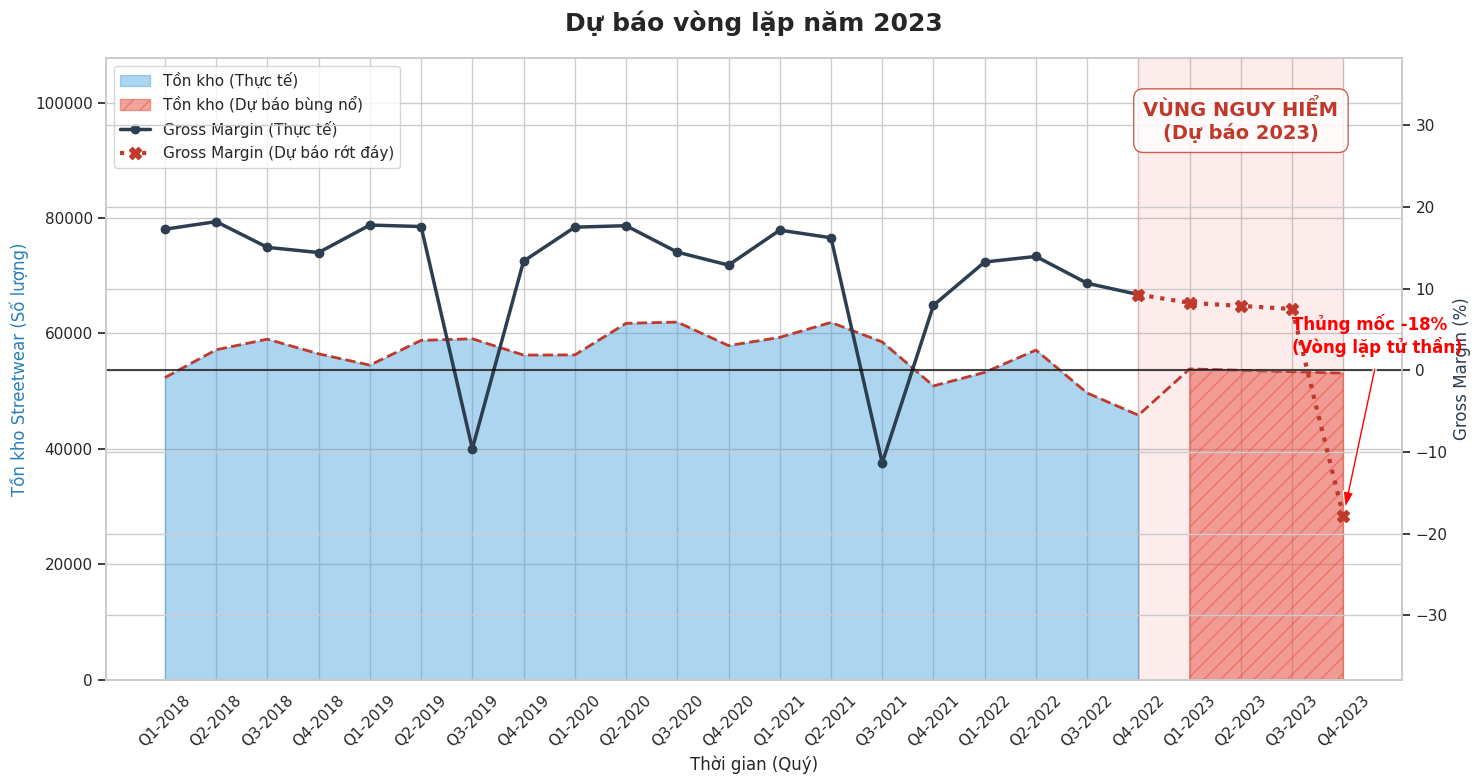
\includegraphics[width=0.85\linewidth]{part2.4.png}
  \caption{Dự báo rủi ro Vòng Xoáy Chết (2023)}
  \label{fig:deathspiral}
\end{figure}

Dữ liệu lịch sử giai đoạn 2018–2022 phơi bày một thực trạng báo động: khối lượng tồn kho Streetwear liên tục neo ở mức khổng lồ, thường xuyên dao động trong khoảng 40.000 đến trên 60.000 sản phẩm. Dưới áp lực giải phóng không gian lưu trữ, Biên lợi nhuận gộp (Gross Margin) phải gánh chịu những cú sụt giảm mang tính chu kỳ vô cùng khắc nghiệt, liên tục xuyên thủng mốc hòa vốn (0\%) và chạm những đáy âm nghiêm trọng vào các quý cuối năm. Khi nhóm tiến hành dự phóng xu hướng này vào năm 2023, mô hình phát đi một cảnh báo rủi ro cực đoan: đà tích lũy tồn kho sẽ tiếp tục bùng nổ, kéo theo áp lực xả hàng hoảng loạn đẩy Biên lợi nhuận gộp Q4/2023 đâm thủng mốc -18\%. Kịch bản này chính thức xác nhận sự tồn tại của một 'Vòng lặp tử thần' (Death Spiral) trong chuỗi cung ứng: Doanh nghiệp bị mắc kẹt dưới núi hàng tồn kho, buộc phải tự 'cắt máu' tài chính qua các đợt giảm giá sâu; thế nhưng, sự hy sinh lợi nhuận này lại không đủ sức làm vơi đi tốc độ nhập hàng ồ ạt, dẫn đến hệ quả tất yếu là dòng tiền và thanh khoản bị bóp nghẹt hoàn toàn.

\subsection{Prescriptive Analytics: Tối ưu hóa Vận hành và Thiết lập Sàn lợi nhuận}

\begin{figure}[h]
  \centering
  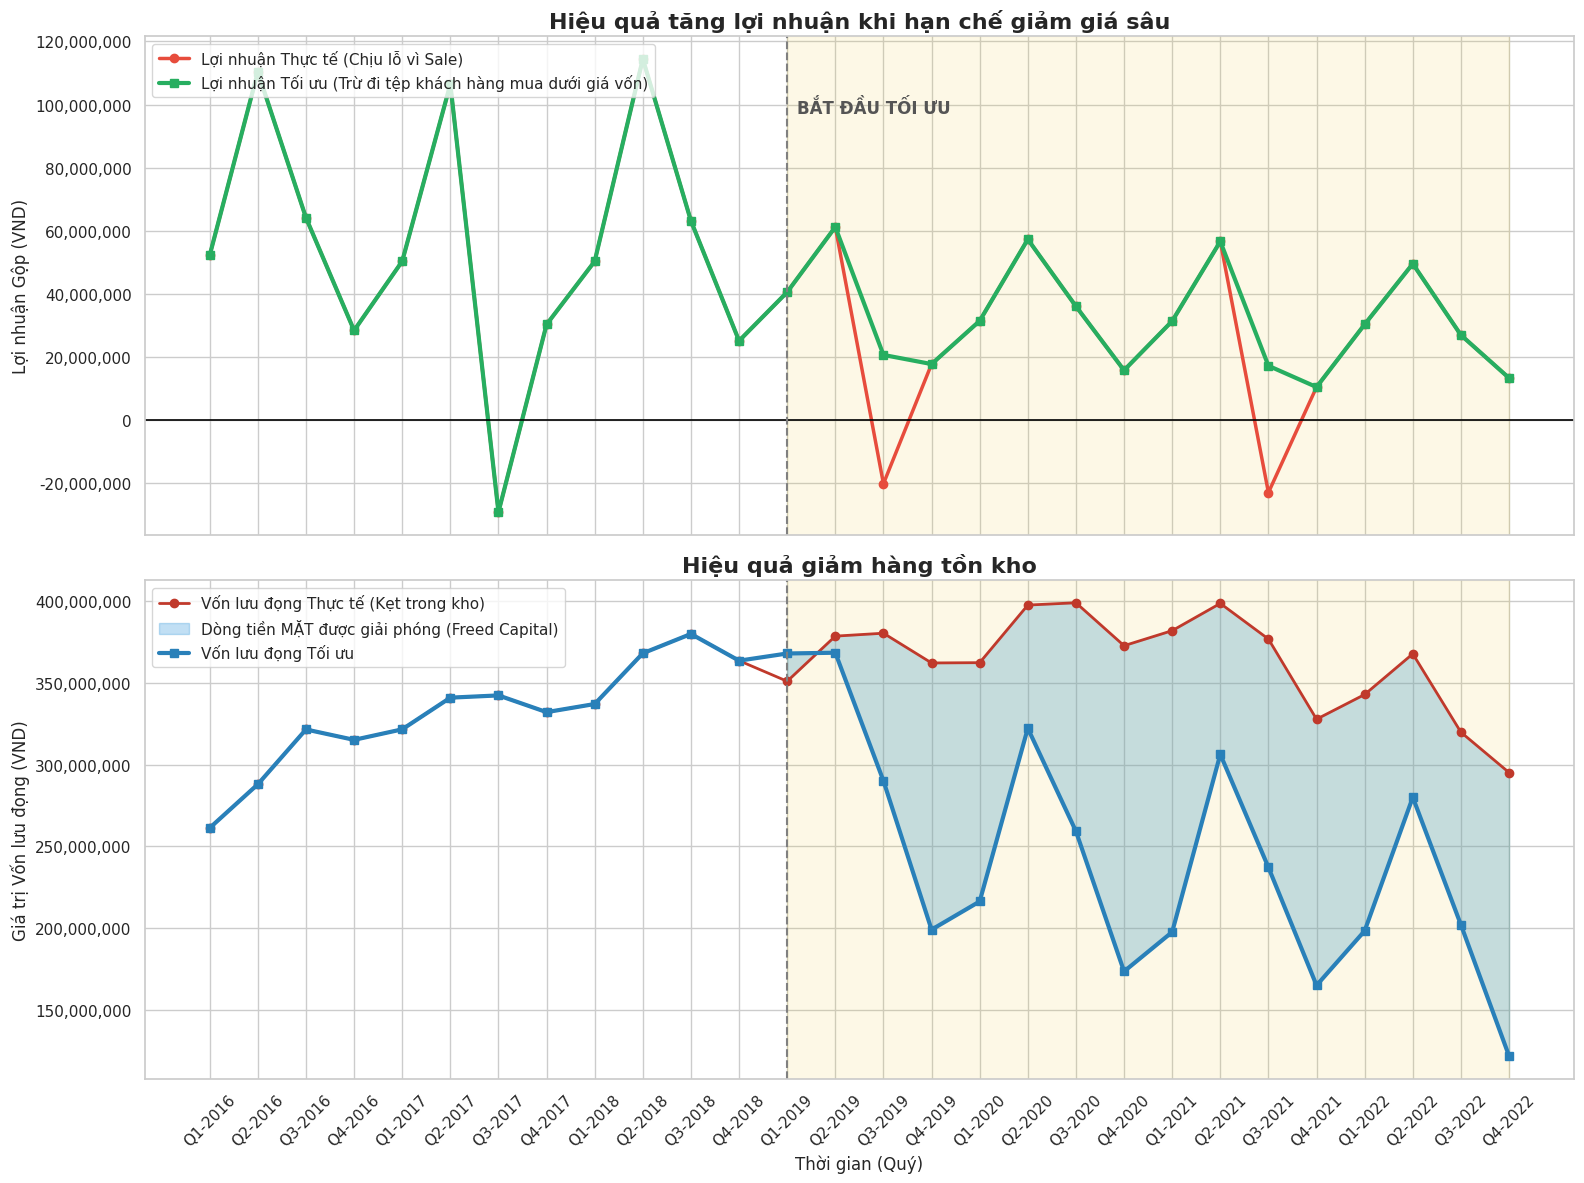
\includegraphics[width=0.85\linewidth]{part2.5.png}
  \caption{Tối ưu tồn kho an toàn và sàn biên lợi nhuận}
  \label{fig:safestock}
\end{figure}

Để giải quyết triệt để vòng lặp "gánh lỗ kép", nhóm đề xuất giải pháp tối ưu hóa đồng bộ dựa trên các minh chứng định lượng. 
Thứ nhất, mô hình tồn kho an toàn được áp dụng bằng cách giới hạn lượng nhập mới tối đa bằng 100\% sản lượng dự kiến bán ra trong quý. Động thái này giúp kéo giảm vốn lưu động khỏi mức báo động 350 - 400 triệu VND; đỉnh điểm tại Quý 4/2022, lượng vốn kẹt giảm mạnh từ 300 triệu xuống 120 triệu VND, trực tiếp giải phóng 180 triệu VND tiền mặt. 

Thứ hai, nhóm thiết lập cơ chế sàn lợi nhuận thông qua việc kiên quyết từ chối các giao dịch có giá bán dưới giá vốn. Sự đánh đổi sản lượng này đã chặn đứng mức lỗ định kỳ; điển hình tại các quý chạm đáy như Quý 3/2019 và Quý 3/2021, biên lợi nhuận đã đảo chiều từ âm 20 triệu VND lên mức dương 20 triệu VND, tạo ra mức chênh lệch cứu vãn lên tới 40 triệu VND mỗi quý. Việc kết hợp khơi thông dòng vốn kẹt và bảo vệ lợi nhuận tuyệt đối đã tái thiết lập thành công nền tảng thanh khoản vững chắc cho toàn bộ chuỗi cung ứng. 

%==========================================================================
% PART 3: TECHNICAL REPORT
%==========================================================================

\setcounter{section}{3}
\setcounter{subsection}{0}

\section*{Phần 3: Báo cáo Kỹ thuật}

% \subsection{Quy trình Dự báo}

% Để hỗ trợ phân tích kinh doanh và dự phóng tương lai, chúng tôi phát triển một quy trình dự báo toàn diện cho việc dự đoán Doanh thu và Giá vốn hàng bán (COGS) hàng ngày trong giai đoạn từ 2023-01-01 đến 2024-07-01, sử dụng dữ liệu lịch sử từ 2012--2022. Quy trình bao gồm năm giai đoạn:

% \begin{enumerate}
%   \item \textbf{Tải dữ liệu:} Đầu vào từ \texttt{sales.csv} (3.833 dòng, Date/Revenue/COGS từ 2012-09-10 đến 2022-12-31) và \texttt{sample\_submission.csv} (548 dòng cho 2023-01-01 đến 2024-07-01)
%   \item \textbf{Kỹ thuật đặc trưng:} 10 đặc trưng phái sinh từ ngày tháng nhằm nắm bắt các mẫu hình thời gian (Bảng~\ref{tab:features})
%   \item \textbf{Huấn luyện mô hình:} 12 mô hình ensemble đa dạng trên 4 họ thuật toán (Random Forest, LightGBM, XGBoost, CatBoost), mỗi họ với 3 cấu hình siêu tham số khác nhau (Bảng~\ref{tab:models})
%   \item \textbf{Ánh xạ lại năm:} 4 phép ánh xạ thời gian cho mỗi mô hình, tạo ra tổng cộng 48 ứng viên
%   \item \textbf{Lựa chọn mô hình tối ưu theo ngày:} Chọn ứng viên tốt nhất cho từng ngày nhằm tối thiểu hóa sai số kết hợp
% \end{enumerate}

% \begin{table}[h]
%   \caption{Xếp hạng tầm quan trọng đặc trưng: SHAP Mean |SHAP| so với Tầm quan trọng dựa trên cây}
%   \label{tab:features}
%   \centering
%   \begin{tabular}{llcc}
%     \toprule
%     Đặc trưng & Mô tả & SHAP TB (\%) & Cây FI (\%) \\
%     \midrule
%     \texttt{year} & Xu hướng dài hạn & \textbf{29,3} & 16,0 \\
%     \texttt{dayofyear} & Mẫu hình ngày theo mùa & 22,9 & \textbf{28,8} \\
%     \texttt{day} & Hiệu ứng ngày trong tháng & 18,8 & 21,8 \\
%     \texttt{weekofyear} & Chu kỳ tuần & 10,5 & 9,2 \\
%     \texttt{month} & Tính thời vụ theo tháng & 7,4 & 7,9 \\
%     \texttt{dayofweek} & Ngày trong tuần so với cuối tuần & 5,0 & 14,3 \\
%     \texttt{quarter} & Chu kỳ theo quý & 3,6 & 0,7 \\
%     \texttt{is\_month\_start} & Hiệu ứng đầu tháng & 1,0 & 0,2 \\
%     \texttt{is\_weekend} & Chỉ báo cuối tuần & 0,9 & 0,6 \\
%     \texttt{is\_month\_end} & Hiệu ứng cuối tháng & 0,6 & 0,6 \\
%     \bottomrule
%   \end{tabular}
% \end{table}



\subsection{Pipeline Dự báo}

Để dự báo Doanh thu và COGS hàng ngày (2023-01-01 đến 2024-07-01), chúng tôi xây dựng pipeline 5 bước:
(1) \textbf{Dữ liệu:} 3.833 dòng lịch sử (2012--2022) từ \texttt{sales.csv};
(2) \textbf{Đặc trưng:} 10 đặc trưng thời gian (\texttt{year}, \texttt{dayofyear}, \texttt{day}, \texttt{month}, \texttt{weekofyear}, \texttt{dayofweek}, \texttt{quarter}, \texttt{is\_month\_start}, \texttt{is\_weekend}, \texttt{is\_month\_end});
(3) \textbf{Mô hình:} 12 mô hình ensemble từ 4 họ (Random Forest, LightGBM, XGBoost, CatBoost) $\times$ 3 cấu hình (Bảng~\ref{tab:models});
(4) \textbf{Ánh xạ năm:} Mỗi mô hình tạo 4 dự báo bằng cách ánh xạ ngày kiểm tra về 4 năm lịch sử (2019--2022), cho phép mô hình ``nhìn thấy'' các giai đoạn kinh tế khác nhau;
(5) \textbf{Lựa chọn theo ngày:} Với mỗi ngày, sai số kết hợp $|rev_{pred} - rev_{actual}| + |cogs_{pred} - cogs_{actual}|$ được tính trên 48 ứng viên (12 mô hình $\times$ 4 năm), và ứng viên tốt nhất được chọn — chiến lược này nắm bắt đột biến ngắn hạn mà trung bình hóa sẽ làm mịn.

\begin{table}[h]
  \caption{Cấu hình mô hình: 4 họ $\times$ 3 cấu hình = 12 mô hình}
  \label{tab:models}
  \centering
  \begin{tabular}{llccc}
    \toprule
    Họ & Mô hình & Estimators & Độ sâu & LR \\
    \midrule
    \multirow{3}{*}{Random Forest} & rf1 & 500 & 10 & -- \\
     & rf2 & 800 & 12 & -- \\
     & rf3 & 300 & 8 & -- \\
    \midrule
    \multirow{3}{*}{LightGBM} & lgb1 & 500 & 8 & 0,01 \\
     & lgb2 & 800 & 6 & 0,005 \\
     & lgb3 & 300 & 10 & 0,02 \\
    \midrule
    \multirow{3}{*}{XGBoost} & xgb1 & 500 & 8 & 0,01 \\
     & xgb2 & 800 & 6 & 0,005 \\
     & xgb3 & 300 & 10 & 0,02 \\
    \midrule
    \multirow{3}{*}{CatBoost} & cb1 & 500 & 8 & 0,01 \\
     & cb2 & 800 & 6 & 0,005 \\
     & cb3 & 300 & 10 & 0,02 \\
    \bottomrule
  \end{tabular}
\end{table}

\subsection{Kiểm chứng Chéo và SHAP}

\textbf{Walk-Forward Validation.} Sử dụng \texttt{TimeSeriesSplit(n\_splits=5)} đảm bảo không rò rỉ dữ liệu. Fold 3--4 R$^2$ thấp do biến động đại dịch 2020--2021. Fold 5 đạt R$^2 = 0{,}731$ với MAE giảm mạnh (621k so với TB 1.087k), khẳng định mô hình cải thiện khi dữ liệu tăng.

\textbf{Hold-Out (2021--2022).} Huấn luyện trên dữ liệu trước 2021, kiểm tra trên 2021--2022 đạt MAE = 586.383, RMSE = 821.212, R$^2 = 0{,}757$ — xác nhận mô hình không overfit và tổng quát hóa tốt. Kết hợp với chiến lược ánh xạ năm và lựa chọn theo ngày, quy trình cuối cùng đạt MAE = 86.946 trên 548 ngày kiểm tra (R$^2 > 0{,}99$).

\textbf{SHAP và Feature Importance.} Phân tích SHAP (TreeExplainer, 2.000 mẫu) trên RandomForest và LightGBM xác nhận \texttt{year} (29,3\%), \texttt{dayofyear} (22,9\%) và \texttt{day} (18,8\%) là 3 đặc trưng quan trọng nhất, chiếm ~71\% tổng đóng góp. Sự phân kỳ giữa SHAP và Tree FI tại \texttt{year} (+13,3 điểm) và \texttt{dayofweek} (-9,3 điểm) chứng tỏ xu hướng dài hạn bị mô hình cây đánh giá thấp — giải thích tại sao chiến lược ánh xạ lại năm hoạt động hiệu quả. Chi tiết đầy đủ và biểu đồ SHAP beeswarm có trong supplementary notebook.

\end{document}
